\section{Gráfica de Proceso (Algoritmo paso a paso)}

En esta segunda etapa del análisis, se evalúa la propagación del error mediante el método de
Gráfica de Proceso o Árbol de Cómputo. A diferencia del método analítico directo, este enfoque
desglosa la fórmula resolvente en una secuencia de operaciones elementales, permitiendo
identificar no solo la propagación de los errores inherentes ($i_a$, $i_b$, $i_c$), sino también
la contribución de los errores de redondeo ($\mu_i$) introducidos en cada paso intermedio por el
sistema de representación. Las expresiones de error que se presentan a continuación fueron
obtenidas mediante la herramienta \texttt{GraficaDeProceso} provista por la cátedra, que emplea
cálculo simbólico para derivar automáticamente los factores de amplificación en cada nodo del
árbol de cómputo.

A lo largo de esta sección se utiliza la notación $D = b^2 - 4ac$ para referirse al discriminante
de la ecuación cuadrática, de modo que $x_{1,2} = \dfrac{-b \pm \sqrt{D}}{2a}$.

% ─────────────────────────────────────────────
\subsection{Análisis para la Raíz \texorpdfstring{$x_1$}{x1}}

Para la raíz $x_1(a,b,c) = \dfrac{-b + \sqrt{b^2 - 4ac}}{2a}$, el cálculo se descompone en la
siguiente secuencia de nueve operaciones elementales, enumeradas desde el índice $0$
(convención de la herramienta):

\begin{equation*}
    \text{op}_i:\quad
    \bigl[b^2,\;4a,\;4ac,\;b^2-4ac,\;\sqrt{D},\;-b,\;-b+\sqrt{D},\;2a,\;x_1\bigr]
\end{equation*}

Cada $\mu_i$ denota el error de redondeo introducido en la operación $\text{op}_i$.
A partir de este desglose la herramienta obtiene las siguientes expresiones:

\begin{itemize}

    \item \textbf{Error Inherente ($x_1$):}

    \begin{equation*}
        e_{inh}(x_1) \approx
        - \frac{2ac \cdot i_c}{D - b\sqrt{D}}
        + i_a \left(- \frac{2ac}{D - b\sqrt{D}} - 1\right)
        + i_b \left(
            \frac{2b^2\sqrt{D}}{8abc - 8ac\sqrt{D} - 2b^3 + 2b^2\sqrt{D}}
            - \frac{b}{-b + \sqrt{D}}
          \right)
    \end{equation*}

    \item \textbf{Error de Redondeo ($x_1$):}

    \begin{multline*}
        e_{red}(x_1) \approx
        - \frac{2ac\,\mu_1}{D - b\sqrt{D}}
        - \frac{2ac\,\mu_2}{D - b\sqrt{D}}
        + \frac{b^2\mu_0\sqrt{D}}{8abc - 8ac\sqrt{D} - 2b^3 + 2b^2\sqrt{D}} \\
        - \frac{b\,\mu_5}{-b + \sqrt{D}}
        + \frac{\mu_3\sqrt{D}}{-2b + 2\sqrt{D}}
        + \frac{\mu_4\sqrt{D}}{-b + \sqrt{D}}
        + \mu_6 - \mu_7 + \mu_8
    \end{multline*}

\end{itemize}

En la Figura~\ref{fig:gp_x1} se muestra el árbol de cómputo resultante. Los nodos circulares
(en verde) representan las variables de entrada con sus errores inherentes $i_a$, $i_b$, $i_c$;
los nodos rectangulares (en rojo) representan las operaciones intermedias con sus errores de
redondeo $\mu_i$; y los valores sobre cada arista corresponden a los factores de amplificación
$\partial\,\text{op}_i / \partial\,\text{op}_j \cdot \text{op}_j / \text{op}_i$.

\begin{figure}[H]
    \centering
    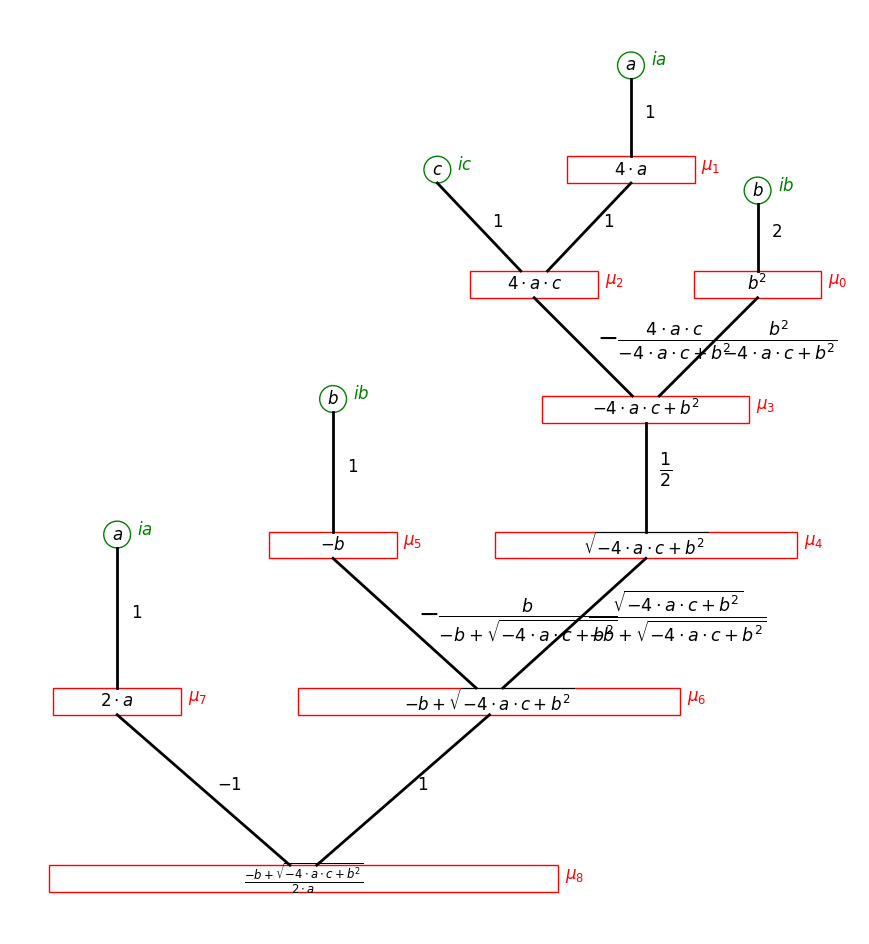
\includegraphics[width=0.9\textwidth]{static/x1_error.png}
    \caption{Árbol de cómputo para el cálculo de $x_1$, con factores de amplificación sobre
             cada arista y errores de redondeo $\mu_i$ indicados en cada nodo intermedio.}
    \label{fig:gp_x1}
\end{figure}

% ─────────────────────────────────────────────
\subsection{Análisis para la Raíz \texorpdfstring{$x_2$}{x2}}

Para la raíz $x_2(a,b,c) = \dfrac{-b - \sqrt{b^2 - 4ac}}{2a}$, la secuencia de operaciones es
idéntica en estructura a la de $x_1$, con la única diferencia en $\text{op}_6$, donde la suma
del numerador se reemplaza por una resta:

\begin{equation*}
    \text{op}_i:\quad
    \bigl[b^2,\;4a,\;4ac,\;b^2-4ac,\;\sqrt{D},\;-b,\;-b-\sqrt{D},\;2a,\;x_2\bigr]
\end{equation*}

Esta diferencia de signo en $\text{op}_6$ modifica los factores de amplificación de las
operaciones que dependen del numerador, dando lugar a las siguientes expresiones de error:

\begin{itemize}

    \item \textbf{Error Inherente ($x_2$):}

    \begin{equation*}
        e_{inh}(x_2) \approx
        - \frac{2ac \cdot i_c}{D + b\sqrt{D}}
        + i_a \left(- \frac{2ac}{D + b\sqrt{D}} - 1\right)
        + i_b \left(
            - \frac{2b^2\sqrt{D}}{8abc + 8ac\sqrt{D} - 2b^3 - 2b^2\sqrt{D}}
            - \frac{b}{-b - \sqrt{D}}
          \right)
    \end{equation*}

    \item \textbf{Error de Redondeo ($x_2$):}

    \begin{multline*}
        e_{red}(x_2) \approx
        - \frac{2ac\,\mu_1}{D + b\sqrt{D}}
        - \frac{2ac\,\mu_2}{D + b\sqrt{D}}
        - \frac{b^2\mu_0\sqrt{D}}{8abc + 8ac\sqrt{D} - 2b^3 - 2b^2\sqrt{D}} \\
        - \frac{b\,\mu_5}{-b - \sqrt{D}}
        - \frac{\mu_3\sqrt{D}}{-2b - 2\sqrt{D}}
        - \frac{\mu_4\sqrt{D}}{-b - \sqrt{D}}
        + \mu_6 - \mu_7 + \mu_8
    \end{multline*}

\end{itemize}

En la Figura~\ref{fig:gp_x2} se muestra el árbol de cómputo correspondiente.

\begin{figure}[H]
    \centering
    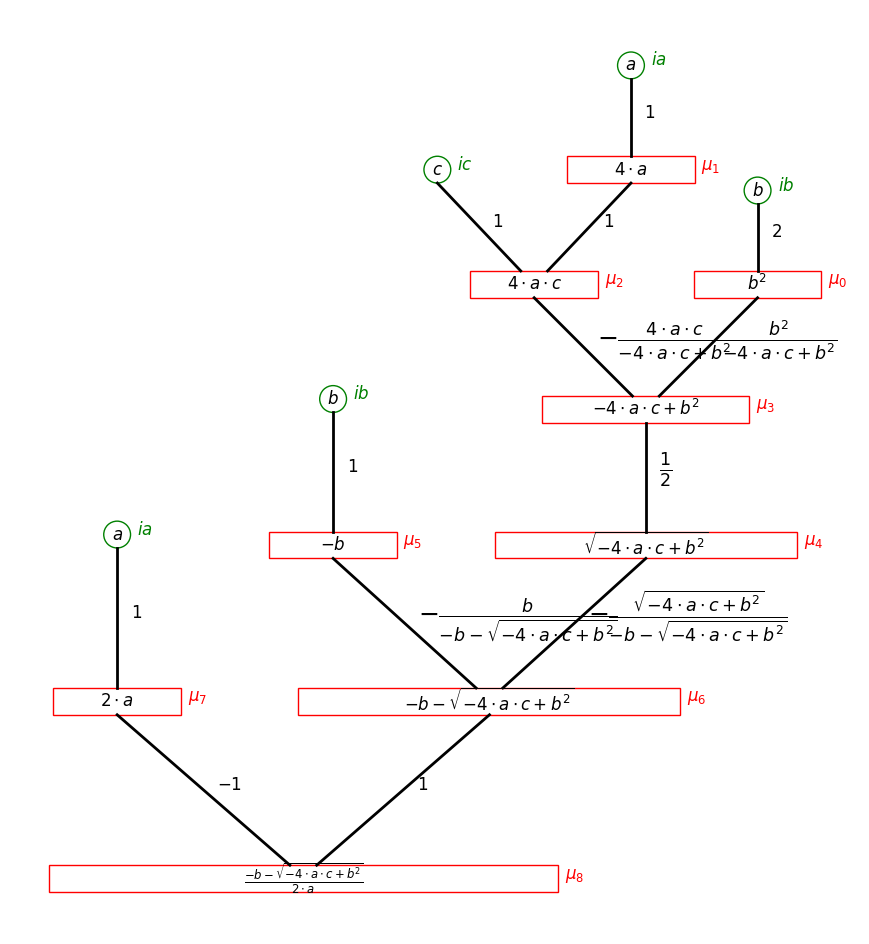
\includegraphics[width=0.9\textwidth]{static/x2_error.png}
    \caption{Árbol de cómputo para el cálculo de $x_2$, con factores de amplificación sobre
             cada arista y errores de redondeo $\mu_i$ indicados en cada nodo intermedio.}
    \label{fig:gp_x2}
\end{figure}

Comparando ambas expresiones se observa que la estructura de $e_{inh}(x_2)$ y $e_{red}(x_2)$
es análoga a la de $x_1$, con la diferencia sistemática de que el denominador $D - b\sqrt{D}$
se reemplaza por $D + b\sqrt{D}$, y los signos de los términos asociados a $\mu_0$, $\mu_3$ y
$\mu_4$ se invierten. En particular, cuando $b > 0$ y $D \approx b^2$ (discriminante cercano a
$b^2$, es decir $4ac \to 0$), el denominador de los primeros términos de $x_1$ se aproxima a
cero, lo que amplifica fuertemente el error inherente de esa raíz. El fenómeno análogo en $x_2$
ocurre cuando $b < 0$, situación en la que $D + b\sqrt{D} \to 0$. Este comportamiento,
conocido como \textit{cancelación catastrófica}, será analizado cuantitativamente en la
sección de comparación.